\section{Conformer-CTC: Non-autoregressive ASR}

\begin{frame}{}
    \LARGE \textbf{Conformer-CTC: Non-autoregressive ASR}
\end{frame}

\begin{frame}{Conformer-CTC Overview}
    \begin{columns}[T,onlytextwidth]
        \begin{column}{0.55\textwidth}
            \begin{itemize}
                \setlength{\itemsep}{1.5em}
                \item \textbf{Conformer:} Combines convolutional and transformer layers.
                \item \textbf{CTC Loss:} Connectionist Temporal Classification for sequence alignment.
                \item \textbf{Non-autoregressive:} Processes entire input sequence in parallel.
            \end{itemize}
        \end{column}
        \begin{column}{0.42\textwidth}
            \begin{center}
                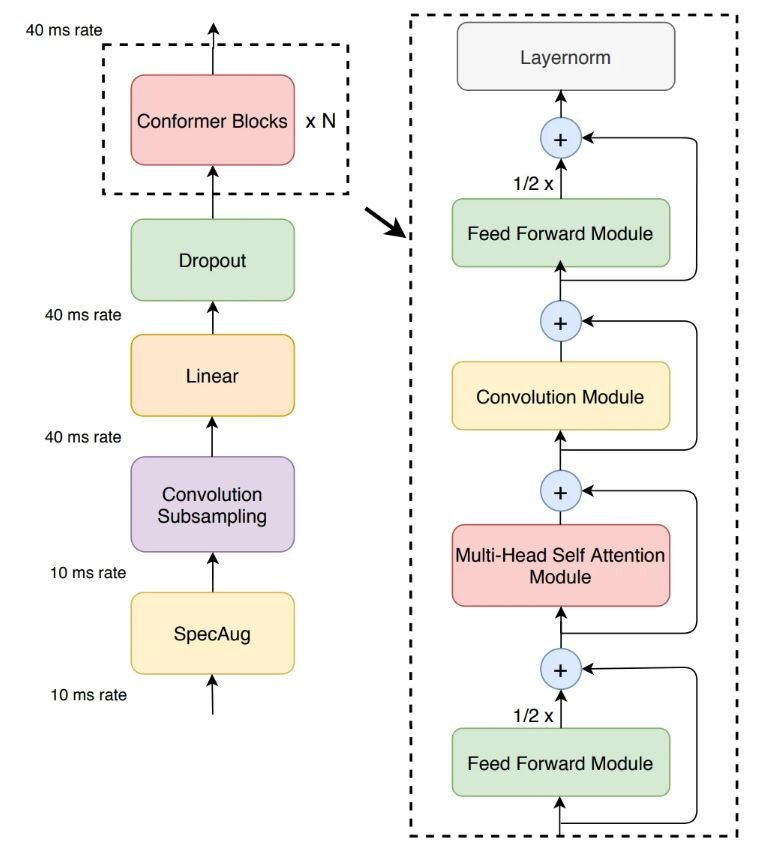
\includegraphics[width=\textwidth,height=0.78\textheight,keepaspectratio]{images/audio-nlp/conformer-ctc.png}\\
                {\scriptsize Source: Gulati et al., ``Conformer,'' Interspeech 2020, Fig.~1.}
            \end{center}
        \end{column}
    \end{columns}
\end{frame}

\begin{frame}{CTC vs Transducer Models}
    \begin{itemize}
        \setlength{\itemsep}{1em}
        \item \textbf{CTC (Connectionist Temporal Classification):}
        \begin{itemize}
            \item Aligns input and output sequences without explicit segmentation.
            \item Every output token is predicted independently, so all frames decode in parallel.
            \item Simpler and faster inference; benefits most from an external language model.
        \end{itemize}
        \item \textbf{Transducer Models:}
        \begin{itemize}
            \item Jointly model alignment and output prediction.
            \item Autoregressive in the output: each token conditions on the previous ones.
            \item Better for streaming and online decoding, since the encoder need not see the whole utterance.
            \item More complex, higher accuracy in some cases.
        \end{itemize}
    \end{itemize}
\end{frame}

\begin{frame}{Conformer-CTC in Production Toolkits}
    \begin{itemize}
        \setlength{\itemsep}{1em}
        \item \textbf{NVIDIA Riva / NeMo:} production ASR toolkits shipping pre-trained Conformer-CTC checkpoints, optimized for GPU inference and both real-time and batch processing.
        \item \textbf{Parakeet:} a family of NeMo models built on a \textbf{FastConformer} encoder, a redesigned Conformer with a more aggressive downsampling schema that runs about $2.8\times$ faster, paired with a CTC, RNN-T, or TDT (token-and-duration transducer) decoder.
        \item \textbf{Citrinet:} a fully convolutional non-autoregressive CTC model, 1-D time-channel separable convolutions plus squeeze-and-excitation, from 9.8M to 142M parameters. Fast because CTC decoding is non-autoregressive; Riva now marks it superseded by Parakeet and Conformer-CTC.
        \item \textbf{References:}
        \begin{itemize}
            \item \href{https://arxiv.org/abs/2005.08100}{Conformer (arXiv:2005.08100)}, \href{https://arxiv.org/abs/2305.05084}{FastConformer (arXiv:2305.05084)}, \href{https://arxiv.org/abs/2104.01721}{Citrinet (arXiv:2104.01721)}
            \item \href{https://docs.nvidia.com/deeplearning/riva/user-guide/docs/reference/models/asr.html}{NVIDIA Riva ASR model docs}
        \end{itemize}
    \end{itemize}
\end{frame}

\begin{frame}{Streaming ASR with SpeechBrain}
    \begin{itemize}
        \item \textbf{SpeechBrain:} open-source toolkit for speech processing.
        \item Supports streaming ASR through a Conformer \emph{transducer} trained with dynamic chunk training, so the encoder only ever sees a bounded chunk of future audio. CTC is kept as an auxiliary loss to stabilise training.
        \item Released streaming checkpoints for LibriSpeech and GigaSpeech.
    \end{itemize}
    \begin{figure}
        \centering
        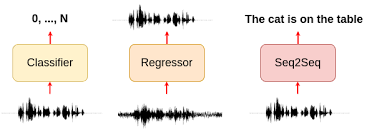
\includegraphics[width=0.85\textwidth,height=0.42\textheight,keepaspectratio]{images/audio-nlp/speechbrain-streaming.png}
        \caption*{\scriptsize The three output shapes SpeechBrain recipes cover: a class label, a continuous value, and a transcript. Source: SpeechBrain (Ravanelli et al., 2021).}
    \end{figure}
\end{frame}

\begin{frame}{Summary: Non-autoregressive ASR}
    \begin{itemize}
        \setlength{\itemsep}{1.5em}
        \item Conformer-CTC enables fast, parallel ASR.
        \item CTC models are simpler and efficient, at the cost of assuming output tokens are independent.
        \item NVIDIA NeMo/Riva and SpeechBrain provide production implementations.
        \item Streaming needs bounded lookahead, which is why streaming recipes usually reach for a transducer rather than plain CTC.
    \end{itemize}
\end{frame}
